\documentclass[10pt,a4paper]{article}

\usepackage[utf8]{inputenc}
\usepackage[french]{babel}
\usepackage[T1]{fontenc}
\usepackage{amsmath}
\usepackage{amsfonts}
\usepackage{amssymb}
\usepackage{hyperref}
\usepackage{graphicx}
\usepackage{caption}
\usepackage{subcaption}
\usepackage[left=2cm,right=2cm,top=2cm,bottom=2cm]{geometry}

\title{Journal de bord}
\author{Gabin Serrurot}

\begin{document}

\maketitle

\begin{enumerate}
    \item \textbf{08/01/2024:}
        \begin{itemize}
            \item J'ai lu le dossier de présentation du projet
            \item J'ai essayé de créer une organisation sur GitHub afin d'avoir tous les codes au même endroit et afin d'éviter d'être dépend les uns des autres
        \end{itemize}
    \item \textbf{09/01/2024:}
        \begin{itemize}
            \item J'ai finalement décidé de ne pas faire une organisation, juste de faire un dossier dans mon compte GitHub et accorder l'accès à Yahya et Andréa afin de tout simplifier. De cette manière, je peux utiliser GitHub Desktop
            \item J'ai commencé le diagramme des cas d'utilisation "Aller à la recherche d’un actif dans l’entrepôt" avec le site \href{https://online.visual-paradigm.com}{visual-paradigm} : figure~\ref{recherche-actif.png1}
            \item J'ai commencé le diagramme des cas d'utilisation "Contrôler le chargement du camion" avec le site \href{https://online.visual-paradigm.com}{visual-paradigm} : figure~\ref{controle-chargement.png1}
            \item Il y aura aussi les diagrammes d'exigences et de déploiement à faire, même s'ils ne sont pas notés dans le dossier de présentation du projet
        \end{itemize}
    \item \textbf{10/01/2024:}
        \begin{itemize}
            \item J'ai d'abord perdu une bonne heure à essayer de debugger mon journal de bord, l'inclusion d'images ne fonctionnait pas alors qu'il manquait juste "usepackage{graphicx}" pour que tout fonctionne.
            \item J'ai repris les diagrammes que j'ai fais la veille avec M. Hacquard : figures~\ref{recherche_actif.png2} et~\ref{controle_chargement.png2} 
        \end{itemize}
    \item \textbf{11/01/2024:}
        \begin{itemize}
            \item Je me suis lancé dans les diagrammes de déploiement mais Pierre m'a dit que ces diagrammes sont à faire par équipe car ils représentent tout le système, pas chacun le sien
            \item J'ai donc décidé de faire la reformulation du cahier des charges
        \end{itemize}
    \item \textbf{12/01/2024:}
        \begin{itemize}
            \item J'ai vu pour la première fois un beacon avec M. Lejoncour
            \item J'ai commencé le cahier de recette
        \end{itemize}
    \item \textbf{15/01/2024:}
        \begin{itemize}
            \item J'ai fais l'IHM de l'application (la veille mais faut pas le dire, cf image)
        \end{itemize}
    \item \textbf{11/01/2024:}
        \begin{itemize}
            \item 
        \end{itemize}
\end{enumerate}

\newpage

\section{Annexes}

\begin{figure}[h!]
    \centering
    \begin{subfigure}[b]{0.45\textwidth}
        \centering
        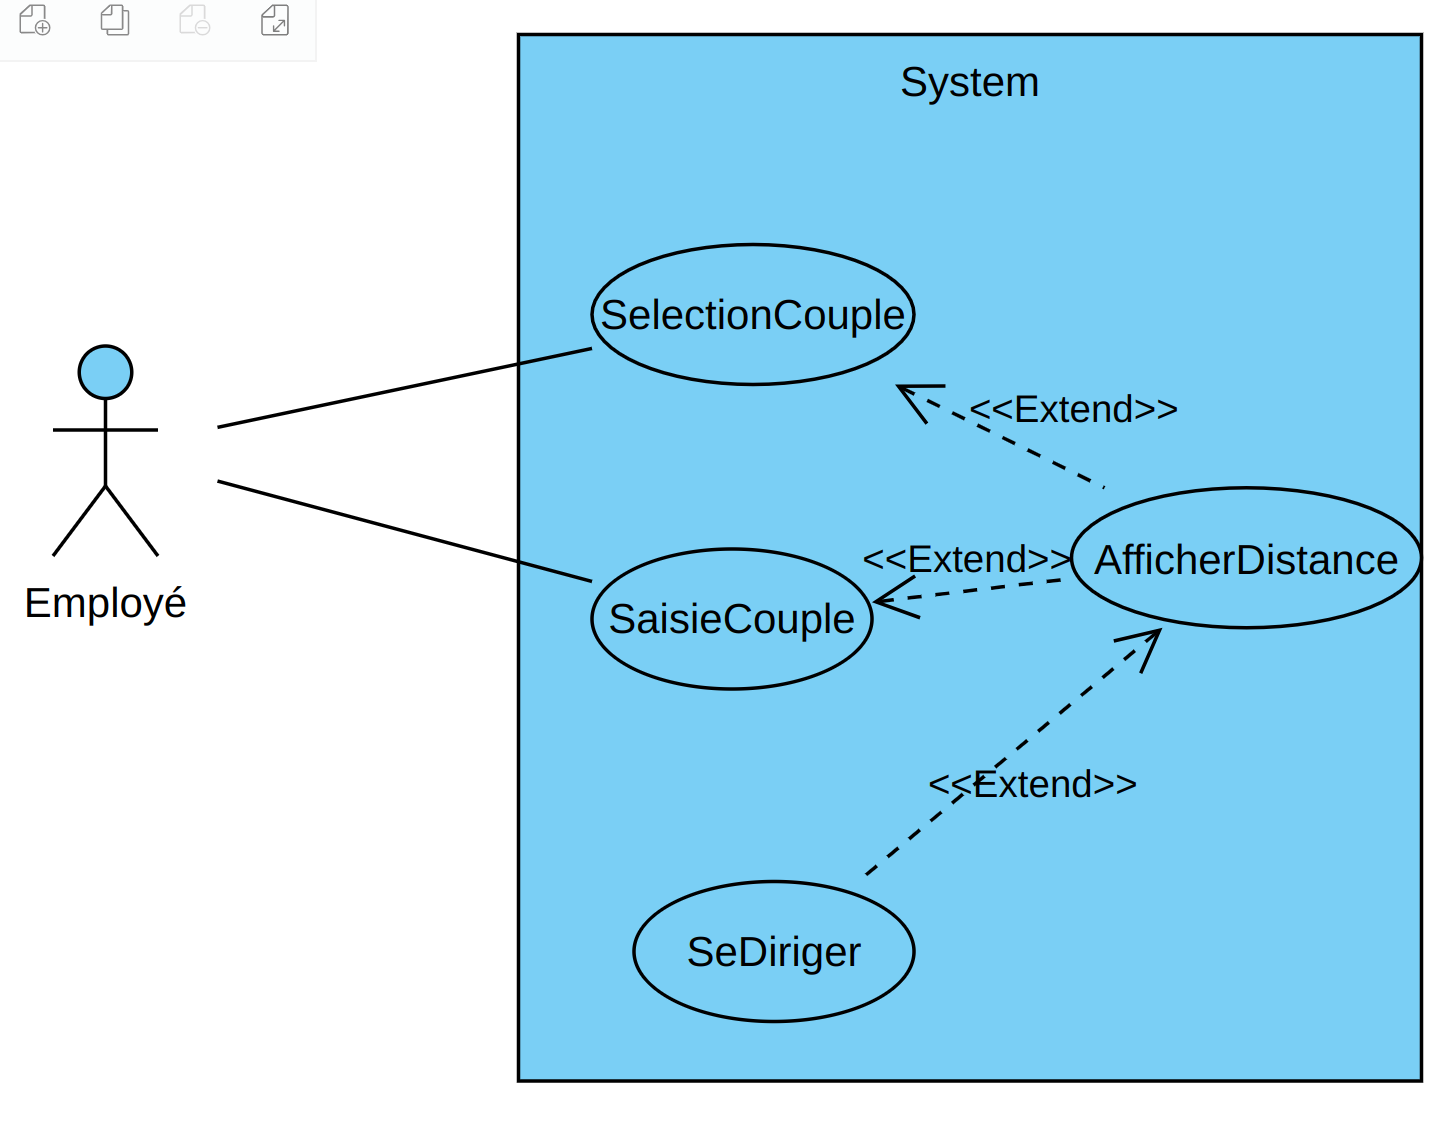
\includegraphics[scale=0.14]{Images/recherche-actif.png}
        \caption{}
        \label{recherche-actif.png1}
    \end{subfigure}
    \begin{subfigure}[b]{0.45\textwidth}
        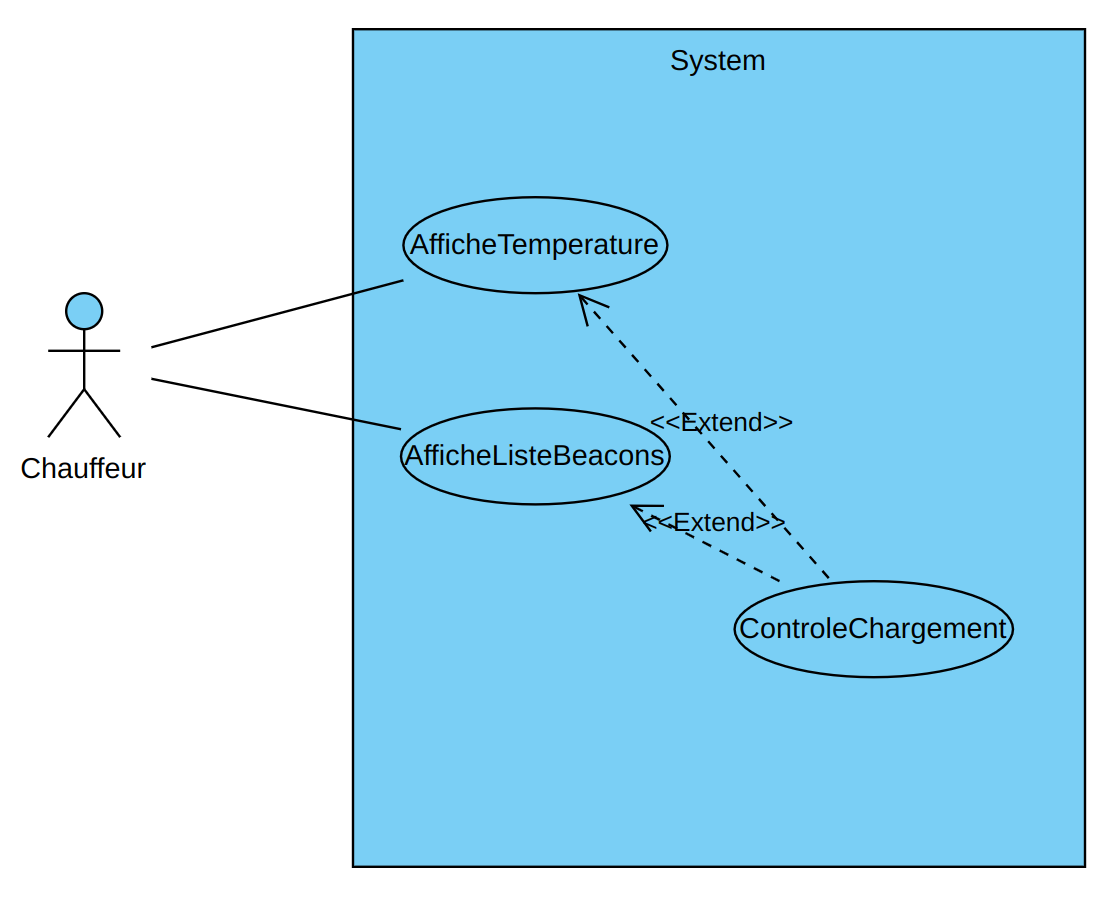
\includegraphics[scale=0.14]{Images/controle-chargement.png}
        \caption{}
        \label{controle-chargement.png1}
    \end{subfigure}
    \caption{}
\end{figure}

\begin{figure}[h!]
    \centering
    \begin{subfigure}[b]{0.45\textwidth}
        \centering
        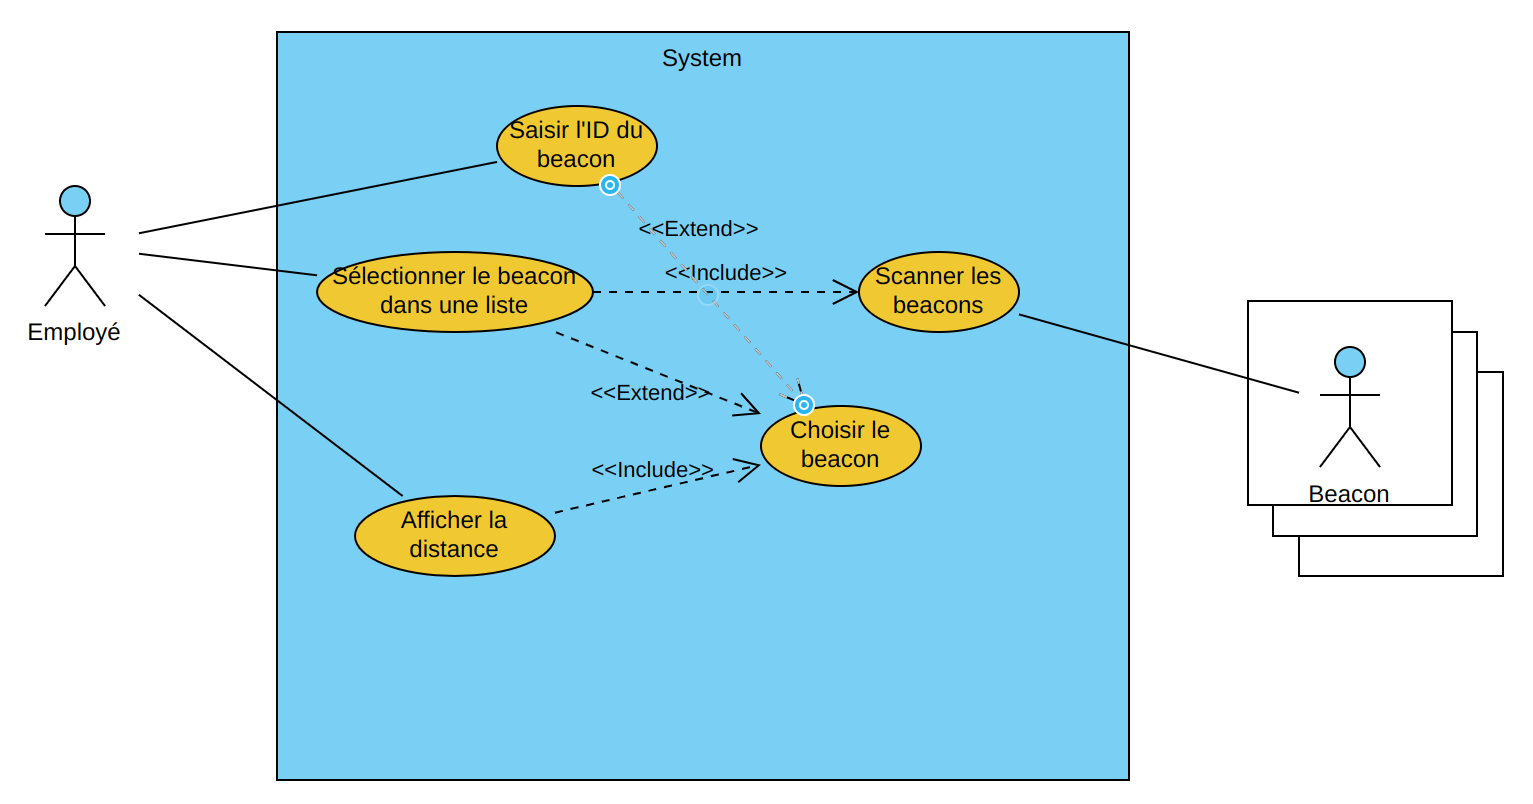
\includegraphics[scale=0.14]{Images/recherche_actif.png}
        \caption{}
        \label{recherche_actif.png2}
    \end{subfigure}
    \begin{subfigure}[b]{0.45\textwidth}
        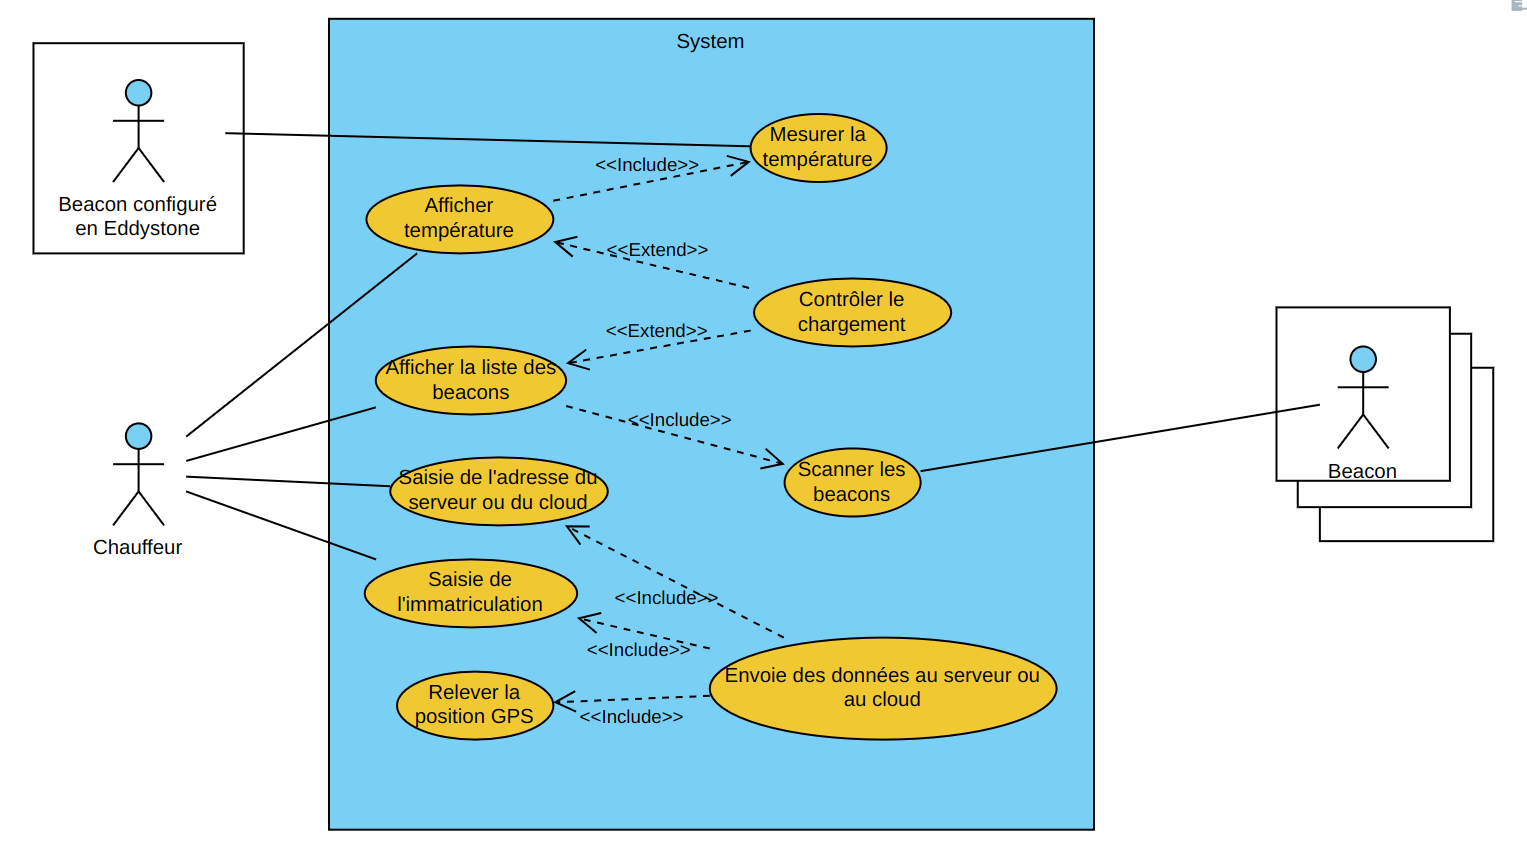
\includegraphics[scale=0.14]{Images/controle_chargement.png}
        \caption{}
        \label{controle_chargement.png2}
    \end{subfigure}
    \caption{}
\end{figure}

\begin{figure}[h!]
    \centering
    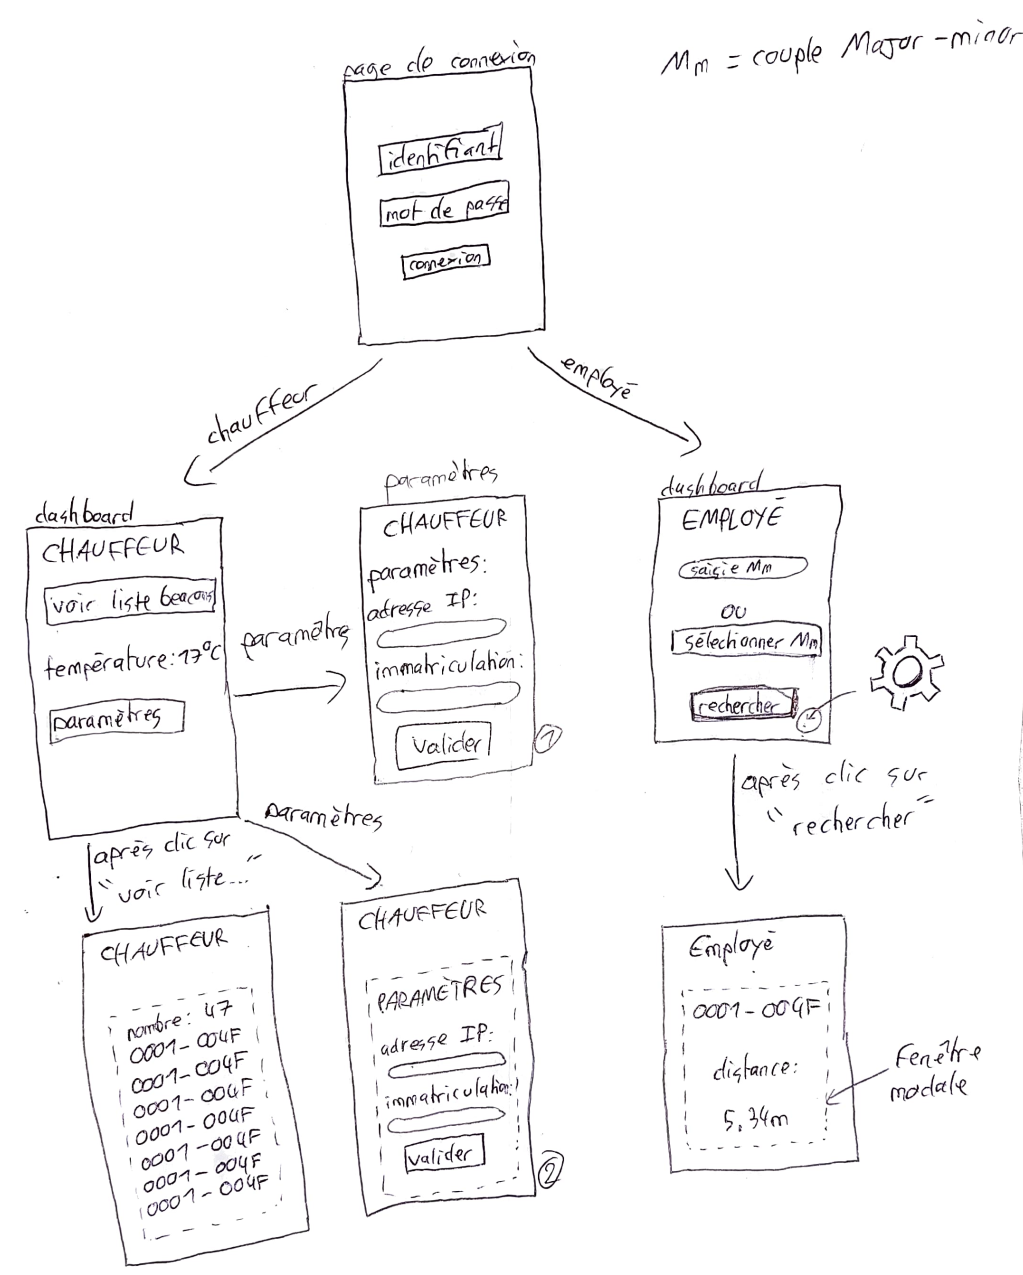
\includegraphics[scale=0.1]{Images/idee_design_application1.png}
    \caption{}
    \label{idee_design_application1}
\end{figure}

\end{document}
